\chapter{Concept}\label{Chap:Concept}

This chapter will explain what requirements were defined for the to be built system and how it will be designed and setup. At first, I will define the goal of this project before writing about the user and system requirements. Then an example Use-Case should help to further understand the goal and purpose of this project.  For further reading, the system will be called "Parametrised Augmented Reality Robot-Human Interface" (\textit{PARRHI}).

\section{Goal, Requirements and Use Cases}
As described in section \ref{Section:PARRHIApproach} this thesis presents a possible approach to solve the previously described problems (see section \ref{Section:ProblemDescription}), which were the difficulty of developing AR applications for users of the robotic industry due to interdisciplinary context. It is the main target of this thesis to remove the necessity of high software engineering skills to develop reasonably complex Augmented Reality Robot-Human Interfaces, maintaining the quality of the outcome and even increasing the degree of reusability. This might result in lower development costs, in a lower struggle to gather software engineering talent and even in a shorter time to market.

To succeed in achieving this goal, a specific set of requirements has to be defined and documented in a formal way.

\subsection{Requirements}\label{Section:Requirements}

Before defining the system's requirements, the end user has to be visualised first. The end user is the person, who develops Augmented Reality applications for industrial systems with the PARRHI system. Application engineers, plant operators or also quality control employees would be fitting users. Employees within these roles have a profound technical background but often do not have any experience with Augmented Reality development or are not software engineers at all.

The PARRHI system should allow these types of end-users to:
\begin{itemize}
	\setlength\itemsep{-1em}
	\item Create AR Applications without any knowledge about AR development (Image Tracking, AR hardware, corresponding engines and frameworks)
	\item Involve their domain-specific knowledge in the application's workflow, content and appearance.
	\item Superimpose the real world with three-dimensional Holograms to describe, highlight or mark real and virtual objects.
	\item Reuse previous work easily since many applications share a very similar base workflow and only vary in smaller details.
	\item Build applications for multiple platforms (Desktop, mobile devices, tables, head-mounted AR devices) 
	\item Have the tools necessary to create medium complex applications for use cases such as tutorials, maintenance instructions or similar tasks.
	\item Have the possibility to control the robot, but also to let the operator take over the controlling at runtime.
	\item Be able to simulate the real and virtual world, to allow development without any hardware being present. 
\end{itemize}

Deriving from these user requirements, the PARRHI system itself should:

\begin{enumerate}
	\setlength\itemsep{-1em}
	\item handle all Augmented Reality aspects without any developer input. This includes position recognition of the AR end user and the robot, the corresponding image and motion tracking and the build process for different hardware platforms.
	\item allow programming and parametrisation in a simple and intuitive, which allows the developer to reuse code from other projects.
	\item allow the definition of 2D/3D objects including the utilisation of the robot's position via simple parameters.
	\item deliver human-readable and intuitive feedback on the written program, comparable to but not exactly compiler error messages, since they are often useless for non-experienced programmers.
	\item support building for multiple platforms such as handheld mobile devices and head-mounted Augmented Reality glasses.
	\item make applications with medium complex workflows (Values in the range of 1-15 following the McCabe Metric~\cite{mccabe1976complexity}) possible. Event-based logic, conditions and actions should be offered.
	\item allow the combination of simulated and real-world data to be used for the application's workflow and its logical operators.
	\item allow the sensing and commanding of the robot's position both relatively and absolutely in joint and task space.
	\item allow documentation of the application's workflow via comments
\end{enumerate}

These basic requirements should be a guideline for further conceptualisation and therefore for the implementation. The next section will visualise one possible use case of the PARRHI System and why it might be interesting to utilise it here.

\subsection{Use-Case example: Factory Maintenance} \label{Section:UseCaseDefinition}

I will now give an example use case, where the PARRHI system is applicable. Bear in mind, that there are more use cases since the PARRHI system is a development environment, which allows a wide variety of workflows. Examples could be AR applications for educational/training purposes, factory workflow processes, investigation and analysis tasks and process profiling.

The Use Case will be explained in the example of a company, which produces its customised products in an agile factory. Plant operators should be supported by an AR app to ensure their safety and efficiency. The factory has highly automated workflows and production lines. Their assembly lines contain robots, which are tasked to prepare the customised parts for the produced products, where each one of them should have different components built into them. The process of mounting and fitting these parts is not fully automated and thus still needs employees to be completed.

Application engineers are now tasked with developing Augmented Reality applications, that support the collaborative process of humans and machines during this assembly step, to increase the safety and efficiency. These engineers have never built AR applications before but have a substantial amount of experience with robot assembly lines and corresponding surveillance applications. The engineers need this application to communicate the intent of robots to the surrounding humans, control the robot to perform its next movement and also ensure, that the collaboration between all parties stays safe, so that neither the human nor robot get damaged. This should be achieved by visually augmenting real-world objects, but also by directly taking over the control of robots.

These engineers now use the PARRHI system to set up AR applications for their respective missions. One, for example, constantly monitors the human's distance to the robot's moving parts and warns the employee visually if they are within the danger zone. At the same time, it always visualises the robot's range of motion and a danger perimeter around its axes, so that the employee has more contextual information to work with. In the case of the human getting too close to the robot, the application immediately stops the robot and commands the user to move away.

The engineers developing these applications can focus on their specific domain knowledge and fill the application with important information, without spending a substantial amount of time with any system setups or framework installations. This use case is exemplary because it reflects a possibly realistic scenario in the real world. Very specific domain knowledge has to be packed into AR applications, where the developers have no experience with AR application development and are under time pressure. 

As I mentioned at the top of this section, there are more use cases for the PARRI system. It is important to notice, that for these use cases no AR specialists are needed since the system takes care of these components. Of course for some use cases, adaptions would have to be made. Certain modules would have to be expanded or adapted for PARRHI to be able to communicate with other machines (see technology transfer section~\ref{Section:TechnologyTransfer}). 

In essence, the majority of work effort can be invested in the application's workflow, which actually solves real-world problems. The surrounding tasks can be ignored since the PARRHI system takes care of them. This is done by people who have no experience in AR development or software engineering in general.

\section{PARRHI Concept}

The following chapter will now explain the concept of the PARRHI system. I will first start with a general overview of the concept and how each requirement is addressed, before shortly explaining each component. After that, the information flow in the system will be elucidated.

Relieving the developer from AR efforts (Reqmt. (1)) means, that the system needs to have all the AR logic implemented on its own, without the need of any developer input. Thus, the architecture has an input and output module, which handle the Augmented Reality aspects. The input module will have to use the AR device's camera to perform the image and motion tracking, and the output module will have to generate the corresponding holograms. The developer's input into the system has to be a document (Reqmt. (2)), which allows the definition of parametrised objects (2D/3D) (Reqmt. (3)) and logic components (Reqmt. (6)). Since the developer needs feedback on their work (Reqmt. (4)), the input document has to be validated. Combining real and simulated world data (Reqmt. (7)) demands the input module to intercept the data stream of the real world, and feed the simulated data into the stream before passing it on. Finally, the in and output modules have to communicate with the robot (Reqmt. (8)).

Fig. \ref{Fig:PARRHIConcept} depicts PARRHI's concept, which attempts to fulfil the given requirements and consists of three main parts. The left-hand side shows the developer, the grey box in the middle is the PARRHI system itself and the right side visualises the environment that surrounds the PARRHI system in both virtual and real space. I will now go into detail and systematically explain each component from (0) to (8), before describing the information flow between them.

\begin{figure}[h]
	\centering
	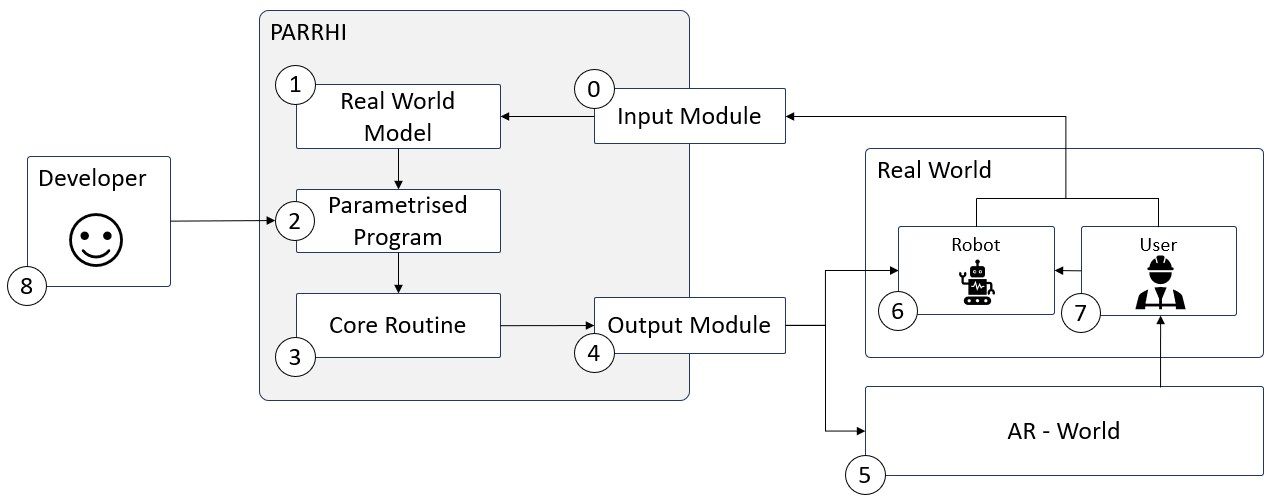
\includegraphics[width=1\textwidth]{Figures/PARRHIConcept03.jpg}
	\caption{PARRHI general concept}
	\label{Fig:PARRHIConcept}
\end{figure}

\begin{enumerate}
	\addtocounter{enumi}{-1}
	\setlength\itemsep{-1em}
	\item Input Module: The Input Module (0) is responsible for collecting data needed from the real world. In this specific case, it receives the robot's (6) joint angles and the user's (7) position.
	\item Real World Model: Since the data from the Input Module (0) might not be in a usable format straight away, it has to be processed first. The Real World Model (1) has a deeper understanding of the real world and helps to extract useful information from the data inflow. This model understanding has to be implemented into the PARRHI system, but could be opened up for parametrisation at a later stage. In this specific case, its outputs are the robot's (6) joint positions and the user's (7) location represented as parameters that are available for the Parametrised Program (2).
	\item Parametrised Program: This is a document that defines the AR application's behaviour and workflow. Its syntax is parametrised, meaning, that it makes use of placeholders (parameters) whose actual value is managed by PARRHI itself at runtime. There are two types of parameters: First, there are the ones that are provided by the Real World Model (1) (for example the discussed robot's (6) joint positions) and secondly any object defined in the Parametrised Program itself (2) can act as a parameter for other objects in the program. These objects can be 3D AR-Hologram definitions, logical instructions or a variety of events and actions. For a more thorough explanation of the Parametrised Program see section \ref{Section:ParametrisedProgram}.
	\item Core Routine: The Core Routine (3) is an interpreter for the Parametrised Program (2), and acts on its instructions. It generates the output of the application, which can either be commands to the robot (6) and thus the real world, or instructions for the AR-World~(5).
	\item Output Module: This component manages the outgoing communication with PARRHI's environment. 
	\item AR-World: The Augmented Reality World is the space, where the AR part of PARRHI's output is displayed. It can contain holograms like spheres and cylinders, but also written text for instructions. The AR-World (5) augments the Real World and is thereby seen by the User (7) through an AR Device.
	\item Robot: It is a Real World object that can be controlled by the User (7) themselves, or by the PARRHI system.
	\item User: This is the person that would use the finished application.
	\item Developer: This person develops the application's workflow and behaviour. Their output is the Parametrised Program (2) as a document, which is validated before being fed into the PARRHI system.
\end{enumerate}

It should now be clearer what each component is responsible for. The following paragraphs will now track the information flow between these components. I will first start with the Developer (8) crafting the Parametrised Document and then continue with the standard cycle of the PARRHI system.

After having defined what the AR-HR-Interface application should achieve, the Developer (8) crafts the Parametrised Program (2). At this point, the Developer pours his domain specific-knowledge and expertise into the system, so that other people like the User (7) can profit from it. The document will be validated first before it is granted access into the PARRHI system. If the validation fails, the Developer (8) receives error messages accordingly and can reiterate over their document until it validates successfully and behaves as the Developer (8) wants it to.

The runtime loop starts with the Input Module (0). It not only collects the robot's (6) joint angles, location and gripper-state but also the User's (7) position. This input data is then fed into the Real World Model (1), which uses its Real World understanding to extract/calculate more useful information. In this specific case, it applies forward kinematics onto the robot's (6) joint angles to calculate their 3D position and transforms the User's (7) location coordinates into PARRHI's internal coordinate system. 

After transforming the input data into a usable format, the placeholders (parameters) in the Parametrised Program (2), are now filled with information by the PARRHI system. For example, the Parametrised Program (2) could use the robot's tool centre point (TCP) for a definition of some AR-holograms, without knowing where exactly the TCP is during development. At runtime, PARRHI inserts this information it received from the Real World Model (1) into the parameters. 

The Core Routine (3) then interprets the now filled-in Program (2). It first updates its internal state with the new parameters, before updating all AR-Holograms. At last, it evaluates all events and triggers their actions if needed. These actions might be commands for the AR-World (5) (for example to show and hide holograms or to change UI text) or commands for the Real World Robot (6) (e.g. to move or stop the robot). These commands are passed on to the Output Module (4), which is responsible for executing them. It has the required tools to communicate with the Robot (6) and with the AR - World (5). 

At this point, the User (7) sees two things. They see the Real World, with the Robot (6) and its surrounding environment, in front of them. The Robot (6) might be instructed to do something by the Output Module (4) already. Superimposed onto the Real World, they also see the Augmented Reality World (5), which contains all visual information that the Output Module (4) constructed. There could be cylindrical translucent holograms marking a danger zone around the robot's (6) axes. The AR-World's (5) content influences the User (7) to do certain things. He could be instructed by holograms to move into a safe-zone. At the same time, the User (7) might control the Robot (6). The Output Module (4) enjoys priority over the User's (7) input when commanding the Robot (6), ensuring the safety of it needs to stop the machine.

As Fig.~\ref{Fig:PARRHIConcept} depicts, the Input Module (0) then finally closes the feedback loop by receiving fresh data from the Real World. The information flow that was followed in the paragraphs above, changed the real world either by direct commands to the robot or indirectly by commanding the User (7) via the AR World (5). These changes will now be reflected in the input data and are thus available for the next cycle. The presented loop repeats itself, where every iteration only takes a fraction of a second until the PARRHI system is terminated for some reason. 

The preceding paragraphs give a relatively detailed overview of the concept behind PARRHI. The following chapters will now explain each part in an even higher degree of detail. The order will be similar to the explanation of the information flow in the PARRHI concept, meaning, that the Input Module (0) and the Real World Model (1) will be explained first, followed by a very thorough explanation of the Parametrised Program (2) with all its objects and definitions. In the end, the Core Routine (3) and the Output Module (4) with the Real and AR-World (5) will finish off the concept chapter.


\subsection{Preparation of Parameters}
One main strength of the \textit{PARRHI} concept is its disclosure of its knowledge of the outside world to its inner components via parameters. Two steps are necessary to do that. First, the Input Module (0) has to automatically retrieve real world information. Since the latter is hard to comprehend for computer programs and might not be usable for the Developer's purpose, the Real World Model (1) processes the input data in some way. Since the preparation of these parameters is an essential part of this concept, the following section will explain their origin, and how they are being prepared for the Parametrised Program. 

The complexity of collecting real-world data strongly depends on the use case. I decided to limit my scope to the collection of three information pieces since it is not the main focus of this thesis. These three pieces are the user's position, the robot's joint angles and it's gripper state. These three information pieces will be fed through the Real-World Model and then be offered as parameters to the Parametrised Program.

To get the user's position, the relative distance and orientation to the robot have to be found first. For AR applications, it is important for the AR device to know its six-dimensional orientation (position and rotation). Otherwise superimposed holograms would not make any sense to the viewer since they appear misplaced. As soon as misplacements of visual augmentations happen, they are more of a distraction than an assistance. To get this relative position, the robot's position has to be received first. This could be done via image tracking. From this vector (user to robot) PARRHI calculates the user's location in the robot's coordinate frame with its model of the real world.

Then the robot's joint positions are needed for the application program to offer the possibility to fully integrate the robot in the application's workflow. Since most robots do not offer their individual joint positions in 3D vectors, but only their joint angles, a corresponding robot model is needed to calculate each joint's position from their joint angles. This is called forward kinematics, an old challenge in robotics with known mathematical tools and ways to solve it (at least in the case of basic industrial robots). In principle, a robot's tool point can be calculated via every joint angle and some knowledge about the robot's configuration. The latter is specified by the types of joints (degrees of freedom (DOF)) and the distance between consecutive joints. A mathematical model then outputs each joint's three-dimensional location, which is offered to the Application Program (2) via parameters. To get an example of how the joint's position might be used in a parametrised way see section~\ref{Section:Points}.

\subsection{Parametrised Program}
\label{Section:ParametrisedProgram}
The Parametrised Program is the document, which the Developer ((8) in Fig. \ref{Fig:PARRHIConcept}) of the PARRHI system produces. It contains parametrised, hierarchically structured data, that defines the behaviour, feel and look of the final AR-HR-application. This document is responsible for fulfilling the defined requirement number (6) in section~\ref{Section:Requirements}, which requires the PARRHI system to allow complex application workflows to be reflected.

The Parametrised Program contains instructions and definitions which from now on will all be called to "objects". All these objects have a certain set of parameters that are needed to fully define their function, visual appearance and behaviour. These parameters can either be previously defined objects, data from the Real World Model or constant values. By using other objects as parameters, one can create an interconnected program with links to other components, where instructions might be able to manipulate other objects in the program at runtime. To reference these other objects, every single object has to have a unique name.

The following chapters explain the set of tools that are available to the developer, how they work and interconnect. Table~\ref{Table:InputDataStructure} displays the different categories of objects. Each section will describe what exactly is parametrised in their definition and how they can be used as parameters to define other program parts.

\begin{table}[ht]
	\caption{\textit{Input Data} structure}
	\label{Table:InputDataStructure}
	\centering
	\begin{tabular}{lcl}
		\toprule
		Name & Section		& Explanation	\\		
		\midrule
		Variables & \ref{Section:Variables}		& Integer variables in a traditional sense \\
		Points& \ref{Section:Points}		& \parbox[t]{10cm}{Different kinds of 3D Point definitions\\(fix, relative to the robot, relative to the user)} 	 \\
		Holograms& \ref{Section:Holograms} & 3D virtual augmentations like spheres and cylinders\\
		Events& \ref{Section:Events} & Tools for logic operations to define workflows \\
		\bottomrule
	\end{tabular}
\end{table}

\subsubsection{Variables}\label{Section:Variables}
Variables are storage locations for numbers and have a symbolic name. When using Variables as parameters, they can be the input and target for instructions and thus take part in the application's logic. With the help of Variables, an application could keep track of something by counting events, or also implement state machines that jump between modes.

\subsubsection{Points}\label{Section:Points}
 
Points essentially are three dimensional vectors ($X$, $Y$, $Z$), with their coordinates being defined using parameters. Depending on the type of Point, different parameters for the definitions are used. There are three types of Points.
\begin{enumerate}
	\setlength\itemsep{-1em}
	\item Fix-Point
	\item Robot-Point
	\item Camera-Point
\end{enumerate}

Points are probably the best example of parametrised information in the PARRHI system. At runtime the data from the Real World Model (see (1) in Fig.~\ref{Fig:PARRHIConcept}) is directly fed into the definition of all points that use the according parameters. Thus, the system updates these objects repeatedly with Real World information, that was fed through the Real World Model. Although points are defined using parameters in some way, points themselves are parameters to other objects in the Parametrised Program.

The \textbf{Fix-Point} has static coordinates and thus fixed values are used to define their coordinate parameters (see figure \ref{InputData:PointFix}). It could be used to set up holograms that visualise certain spacial environmental constraints that do not move.\\Definition Parameters: \textit{name : string, X : float, Y : float, Z : float}.

\textbf{Robot-Points} are defined by two indexes of the robot's joints and one scalar value (see figure~\ref{InputData:PointRobot}). The application's developer does not have to understand the robot's kinematics and simply uses the joint-indexes as parameters. At runtime, the \textit{PARRHI} system retrieves the robot's joint position, uses the Real World Model to calculate each joint's position ($J_0 - J_5$) and then feeds this data into the Robot-Points. The final point's position $P$ is calculated as follows (with s being the scalar value and $J_n$ the position vector of Joint $n$):
\begin{equation}
\boldsymbol{P} = \boldsymbol{J_1} + (\boldsymbol{J_2}-\boldsymbol{J_1}) * s
\end{equation}

As can be seen, the scalar value linearly interpolates between the two joint positions and thus allows for a wider variety of Robot-Points.\\Definition Parameters: \textit{name : string, J1 : int, J2 : int, Scale : float}.

\textbf{Camera-Points} are a way to involve the user's position in the application. Similarly to Robot-Points, the PARRHI system repeatedly retrieves the camera's coordinates via the Input Module, feeds it through the Real World Model to map it onto the internal coordinate systems and finally updates the Camera-Points with the new position data of the head mounted AR-Device. Since there is only one Camera in the PARRHI system, its only parameter is the point's \textit{name : string}.


\begin{figure}[!h]
	\begin{minipage}{0.45\textwidth}
		\centering
		

\tdplotsetmaincoords{60}{120} 
\begin{tikzpicture} [scale=0.01, tdplot_main_coords, axis/.style={->, black, thick}, 
vector/.style={-stealth,black,thick}, 
vector guide/.style={dashed,gray,thin}]

%standard tikz coordinate definition using x, y, z coords
\coordinate (O) at (0,0,0);

%tikz-3dplot coordinate definition using x, y, z coords

\pgfmathsetmacro{\ax}{100}
\pgfmathsetmacro{\ay}{100}
\pgfmathsetmacro{\az}{200}
\pgfmathsetmacro{\axSize}{200}

\coordinate (P) at (\ax,\ay,\az);

%draw axes
\draw[axis] (0,0,0) -- (\axSize,0,0) node[anchor=north east]{$x$};
\draw[axis] (0,0,0) -- (0,\axSize,0) node[anchor=north west]{$y$};
\draw[axis] (0,0,0) -- (0,0,\axSize) node[anchor=south]{$z$};

%draw a vector from O to P
\draw[vector] (O) -- (P);

%draw guide lines to components
\draw[vector guide]         (O) -- (\ax,\ay,0);
\draw[vector guide] (\ax,\ay,0) -- (P);
\draw[vector guide]         (P) -- (0,0,\az);
\draw[vector guide] (\ax,\ay,0) -- (0,\ay,0);
\draw[vector guide] (\ax,\ay,0) -- (0,\ay,0);
\draw[vector guide] (\ax,\ay,0) -- (\ax,0,0);
\node[tdplot_main_coords,anchor=north]
at (\ax+100,0,-60){(\ax, 0, 0)};
\node[tdplot_main_coords,anchor=west]
at (0,\ay,50){(0, \ay, 0)};
\node[tdplot_main_coords,anchor=south]
at (0,0,\az+50){(0, 0, \az)};
\end{tikzpicture}
		\caption{Fix-Point example}
		\label{InputData:PointFix}
	\end{minipage}\hfill
	\begin{minipage}{0.45\textwidth}
		\centering
		
\tdplotsetmaincoords{60}{120} 
\begin{tikzpicture}  [scale=0.03, tdplot_main_coords, axis/.style={->, black, thin}, 
vector/.style={-stealth,green,very thick}, 
robot/.style={green, very thick},
vector guide/.style={dashed,gray,thin}]

%standard tikz coordinate definition using x, y, z coords
\coordinate (O) at (0,0,0);

%tikz-3dplot coordinate definition using x, y, z coords


\pgfmathsetmacro{\axSize}{100}
\pgfmathsetmacro{\jointRadius}{50}

%Robot Points in cm (mm too large dimensions for library)
\coordinate (P0) at (0,0,0);
\coordinate (P1) at (5,0,33);
\coordinate (P2) at (5, 0, 77);
\coordinate (P3) at (15, 0, 100.5);
\coordinate (P4) at (47, 0, 100.5);
\coordinate (P5) at (55, 0, 100.5);
\coordinate (P6) at (63, 0, 100.5);
\coordinate (Point) at (5, 0 , 60);


%draw coordinate system axes
\draw[axis] (0,0,0) -- (\axSize,0,0) node[anchor=north east]{$x$};
\draw[axis] (0,0,0) -- (0,\axSize,0) node[anchor=north west]{$y$};
\draw[axis] (0,0,0) -- (0,0,\axSize) node[anchor=south]{$z$};

%draw the robot's joints and axes
\draw[robot] (P0) -- (P1); \fill[fill=gray] (P0) circle (\jointRadius pt);
\draw[robot] (P1) -- (P2); \fill[fill=gray] (P1) circle (\jointRadius pt);
\draw[robot] (P2) -- (P3); \fill[fill=gray] (P2) circle (\jointRadius pt);
\draw[robot] (P3) -- (P4); \fill[fill=gray] (P3) circle (\jointRadius pt);
\draw[robot] (P4) -- (P5); \fill[fill=gray] (P4) circle (\jointRadius pt);
\draw[robot] (P5) -- (P6); \fill[fill=gray] (P5) circle (\jointRadius pt);

%Draw PointRowot
\fill[fill=black] (Point) circle (\jointRadius pt);

%draw the 
\node[tdplot_main_coords,anchor=east]
at (P1){(Joint 1)};
\node[tdplot_main_coords,anchor=west]
at (P2){(Joint 2)};
\node[tdplot_main_coords,anchor=west]
at (Point){(Point scalar = 0.6)};




\end{tikzpicture}
		\caption{Robot-Point example}
		\label{InputData:PointRobot}
	\end{minipage}
\end{figure}

\subsubsection{Holograms}\label{Section:Holograms}
The AR World can be filled with numerous holograms. In the Parametrised Program these holograms are defined using parameters. In this case, Points from section~\ref{Section:Points} are used to define the Hologram's location and orientation. Since Points are parametrised themselves and are updated by the data from the Real World model, holograms are indirectly also updated regularly.

Holograms in the PARRHI system have a number of attributes (see table~\ref{Table:HologramAttributes}). Currently, \textit{PARRHI} supports two types of holograms. There are spheres and cylinders, respectively taking one or two points and a radius as input parameters to define its size and position. Other attributes describe their visual appearance.

\begin{table}[!htbp]
	\caption{Hologram attributes}
	\label{Table:HologramAttributes}
	\centering
	\begin{tabular}{lll}
		\toprule
		Attribute & Possible values		& Explanation	\\		
		\midrule
		name & any text & Used to identify the object \\
		visibility & visible, hidden & Sets the hologram's visibility \\
		renderMode & normal, transparent & \parbox[t]{10cm}{ normal: Hologram is rendered as a solid object \\ transparent: Hologram is rendered translucent}\\
		radius & number & The radius of the sphere or cylinder \\
		point1 & name of any defined point & Used for the holograms position definition \\
		point2 & name of any defined point & \parbox[t]{10cm}{ Used for the cylinder's position definition \\ (not available for spheres)} \\
		\bottomrule
	\end{tabular}
\end{table}

A Sphere's centre is always equal to its point of definition (\textit{point1}), whereas a cylinder always connects the two points of its definition (\textit{point1} and \textit{point2}). All described types of points in section~\ref{Section:Points} can be used as input parameters for the location. This is the first example of Parametrised Program internal use of objects as parameters.

Holograms have an attribute called \textit{renderMode}, which if set to "transparent", renders the hologram in a half transparent way, allowing holograms to be used for boundary or zone visualizations. Furthermore, the visibility of holograms can be changed by setting the \textit{active} parameter, which is done by actions as described in section~\ref{Section:Events}.

\subsubsection{Events}\label{Section:Events}
All previous elements (variables, points and holograms) exist to define the scene and to set up assets that can be utilised by events, which now actually describe the application's workflow. There are two subtypes in this category. There are event-triggers and event-actions (or short \textit{triggers} and \textit{actions}). Triggers have a boolean expression, which is checked periodically. As soon as the boolean expression evaluates to \textit{true}, the attached actions will be executed and the trigger will be disabled, avoiding multiple executions. One could say that if triggers are \textit{PARRHI's} sensors, then actions are its actuators.

Although there are different types of triggers, all definitions of them have some attributes in common, which are listed in the table~\ref{Table:TriggerAttributes}. Of course, specific trigger types have additional parameters to define their function.

 \begin{table}[!h]
 	\caption{Trigger attributes}
 	\label{Table:TriggerAttributes}
 	\centering
 	\begin{tabular}{lll}
 		\toprule
 		Attribute & Possible values		& Explanation	\\		
 		\midrule
 		name & any text & Used to identify the object \\
 		canTrigger & true, false		& Enables/Disables the trigger \\
 		actions & multiple names of actions & Defines the payload of the trigger \\
 		\bottomrule
 	\end{tabular}
 \end{table}

To reach a reasonable capability, there different and easy to understand triggers are available for the application's developer. In table~\ref{Table:Triggers} is a complete list of all defined triggers.

 
 \begin{table}
 	\caption{Trigger types}
 	\label{Table:Triggers}
 	\centering
 	\begin{tabular}{lll}
 		\toprule
 		Name & Input Parameters		& Trigger expression	\\		
 		\midrule
 		Distance trigger & Two Points $\boldsymbol{P_1}, \boldsymbol{P_2}$, distance $d$		&  $|\boldsymbol{P_2}-\boldsymbol{P_1}| \le d$ \\
		Variable trigger & Variable $v$, trigger value $v_{tr}$ 		& $v = v_{tr}$	 \\
		Time trigger & trigger time $t_{tr}$, time since enabling $t_{enabled}$ & $t_{tr} \geq t_{enabled}$\\
		\bottomrule
	\end{tabular}
\end{table}

\textbf{Distance triggers} are mainly defined using two Points and a distance value. They trigger, as soon as the Euclidean distance of the two points is below the distance parameter. They can be used for two main purposes. First, the application can use the robot's movement as an input using a \textit{Robot-Point}. An action could be triggered as soon as the robot's TCP moves near a wished target point by using a \textit{Fix-Point}. Second, the user's movement can be monitored by using a \textit{Camera-Point} as an input parameter. The application can thus ask the user to move to a specific location (e.g. a safe-zone).\\Definition Parameters: \textit{name:string, canTrigger:bool, point1:Point, point2:Point, distance:float, actions:[Action] }

\textbf{Variable triggers} are defined using a variable parameter, and one \textit{trigger value} parameter. They trigger, as soon as the given variable equals the \textit{trigger variable}. A counter for certain events could be implemented, and trigger an action when a threshold value is reached. It can also be used for workflows that need states or steps. \\Definition Parameters: \textit{name:string, canTrigger:bool, varName:Variable, triggerValue:int, actions:[Action]}

Finally the \textbf{Time trigger} allows the application to involve timers. These triggers are defined using a \textit{timeSinceActivation} parameter and trigger, as soon as the time passed since setting \textit{canTrigger} to true is equal or greater than the \textit{timeSinceActivation} value. If \textit{canTrigger} is true from the beginning on, the timer starts immediately. The user could be given a maximum time for a task or holograms can be hidden after a few seconds.\\Definition Parameters: \textit{name:string, canTrigger:bool, timeSinceActivation:int, actions:[Action]}

Whenever a trigger's boolean expression evaluates to true, its actions are invoked and the trigger gets disabled. There are six different types of actions - each serving a specific purpose. As with triggers, actions have a set of input parameters they need to fulfil their task and to be completely defined. The table~\ref{Table:Actions} gives an overview over all actions that \textit{PARRHI} currently supports.

\begin{table}
	\caption{Event Actions}
	\label{Table:Actions}
	\centering
	\begin{tabular}{lll}
		\toprule
		Action Name & Input Parameter		& Explanation	\\		
		\midrule
		Increment Counter  	& Variable $v$					& Increments the value of $v$ by 1 \\
		Set Hologram State 	& Hologram-names, State to set	& Enables/disables all specified holograms \\
		Set Trigger State  	& Trigger-names, State to set  	& Enables/disables all specified triggers \\
		Change UI Text	  	& Text to set					& Sets the UI Text\\
		Move Robot			& Point $P$						& Moves the robot to $P$ \\
		Set robot-hand State & State to set (open/close)		& Opens or closes the robot's gripper \\
		\bottomrule
	\end{tabular}
\end{table}

\textbf{Increment-counter actions} increment the value of the Variable parameter by 1. If a developer wanted to count the number of times a user jogged the robot into a specific region, an Increment-counter action could be used as a payload of a Distance trigger. After a threshold value is reached, a Variable trigger could change the UI text and display a hint.\\Definition Parameters: \textit{name:string, intVar:Variable}

The \textbf{Set-Hologram-State action} allows the visibility of holograms to be changed at runtime. If a hologram represented a region for a tutorial step, it could be hidden after the user's task was completed. The new scene could then be set up by displaying new holograms that guide the user's way. Another possible scenario would be, to display a warning boundary, if the user moves into a forbidden zone.\\Definition Parameters: \textit{name:string, onHolograms:[Hologram], offHologram=[Hologram]}

When using PARRHI applications the user is presented a GUI that shows text. The \textbf{Change-UI-Text action} allows the changing this displayed text. There are numerous obvious scenarios where this is useful. Whenever it is of value to inform the user about something that cannot be achieved by holograms, this is a simple way to do so.\\Definition Parameters: \textit{name:string, text:string}

To create meaningful and longer applications, enabling and disabling triggers is an essential tool. This is what the \textbf{Set-Trigger-State action} is for. Triggers can only invoke their payload actions, if their attribute \textit{canTrigger} is true. Triggers can either be defined as disabled from the beginning on or automatically get disabled by triggering. The Set-Trigger-State action enables or disables the trigger, which is referenced by the \textit{triggerName} parameter. There is a speciality in the case of \textit{Time triggers}. Their inner timer starts ticking, whenever they get enabled. This allows for timers to be used in the middle of applications, relative to other events.\\Definition Parameters: \textit{name:string, triggerName:Trigger, canTrigger:bool}

The last two actions are designed to take active control over the robot. The \textbf{Move-Robot action} moves the robot to the specified coordinates. It is important to note, that this action has two different modes defined by a \code{mode} parameter. If \textit{mode} is \textit{'t'}, then the coordinates will be interpreted as absolute euclidean task space coordinates, and if \textit{mode} equals \textit{'j'} then PARRHI will assume that the coordinates are defined in joint-space and will act accordingly. Instead of defining the target parameter by a six-dimensional vector, a \textit{Point} reference can also be passed into this parameter.\\Definition Parameters: \textit{name:string, target:Vector6, mode:char}

The \textbf{Set-Robot-Hand-State action} behaves as one would expect and simply open or close the robot's gripper according to its parameters \textit{state}.\\Definition Parameters: \textit{name:string, state:bool}

\subsubsection{Program example}
To further explain the parametrised program, I want to give a short example of how such a small program might be set up. The following program will wait for the user to move the robot's tool centre point (\textit{TCP\_Point}, line 3) to the \textit{Target\_Point} (line 2) at some static coordinates and visualise both points with Sphere holograms (lines 6,7). Upon reaching the target with a certain tolerance (line 10), it will display a success message to the user (line 13).

\begin{lstlisting}
<!-- Define Points -->
<PointFix name="Target_Point" X="200" Y="200" Z="200" />
<PointRobot name="TCP_Point" J1="6" J2="6" scale="0"/>

<!-- Define Holgorams -->
<Sphere name="Target_Area" radius="15" point="Target_Point"/>
<Sphere name="TCP_Area" radius="15" point="TCP_Point"/>

<!-- Define Trigger -->
<DistanceTrigger name="d_trigger" point1="TCP_Point" point2="Target_Point" actions="SetUI_Success" distance="15"/>
	
<!-- Define Action -->
<ChangeUITextAction name="SetUI_Success" text="You have reached your target successfully!"/>
\end{lstlisting}


\subsection{Core Routine}
The Core Routine's responsibility is, to interpret and execute the Parametrised Program. Its input is the Parametrised Program with all data from the Real World Model already set, and it's outputs are commands to the Real or AR World. At the very beginning of each cycle in the Core Routine, all Parameters are resolved (see (0) in Fig.~\ref{Fig:CoreRoutine}). This means, that the interpreter finds all parameters that are used in the Parametrised Program, and inserts all values from the referenced objects. For example, if a Hologram is defined using a Point object, the interpreter looks for the point and fetches its momentary coordinates to fully define the hologram. Similarly, all other parameters are found and processed.

After that, the Core Routine updates its inner state (1). This means, that it updates all Holograms and Triggers with newly received data. Holograms are moved to their new position, and Triggers receive their new input values depending on the Trigger type. Distance Triggers, for example, receive the new coordinates that they monitor.

With all values updated, it can now check all \textit{Triggers} whether or not their boolean expression evaluates to \textit{true} (2). Whenever a \textit{Trigger} does evaluate to true, it invokes all \textit{actions} of that trigger(3). The executing \textit{actions} result in a group of commands, that will be sent to the Output Module, which then handles them from now on. 

\begin{figure}[!h]
	\centering
	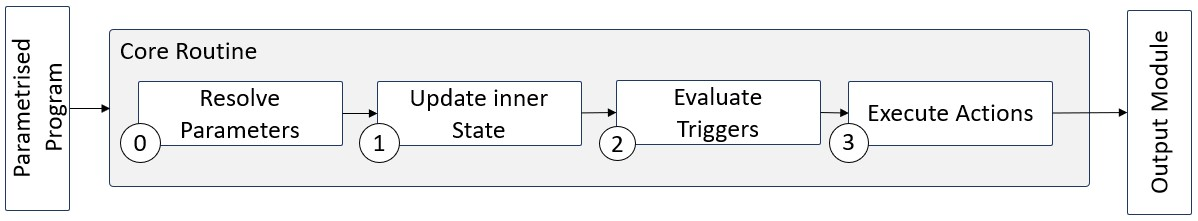
\includegraphics[width=0.85\textwidth]{Figures/CoreRoutine.jpg}
	\caption{Core Routine Workflow}
	\label{Fig:CoreRoutine}
\end{figure}

\subsection{I/O Modules}

The last step in the PARRHI runtime cycle is to send all generated commands to their receivers. As described, there are two types of commands. Firstly, there are the ones that are directed to the AR-World and secondly, there are commands that a directed towards the Real World. I will now shortly explain the difference in their nature, and why AR-commands are much easier to process conceptually than Real World commands.

The AR-World is \textit{only} software that runs on the same device, which hosts the complete PARRHI system. That means, that sending commands to the AR-World is as simple as actually calling some methods in the Back-End. Real World commands, on the other hand, are much more complex because they have to be sent to other hardware devices, with possibly different operating systems (OS) that run on different programming languages. This is why some network protocols have to be defined to communicate with these Real World objects. 

In my case, the Robot (see (6) in fig.~\ref{Fig:PARRHIConcept}) is the only Real World object, that does not run on the same OS as the AR-Device. This means, that an OS neutral protocol has to be defined for this type of communication. In addition to that, operating systems on Robots tend to be sealed towards the outer world securing it against unwanted access but, at the same time, hard to interconnect to other systems. To get more information about the implementation regarding this component see section~\ref{Section:RobotLibrary}.


























